\lecture{3}{4 May 2022}{}
\section{Euler-Lagrange Equations}
If we want to extremize the functional
\begin{equation}
    F[y] = \int_{\alpha}^{\beta} f(x, y, y') \dif x.
    \label{eleq}
\end{equation}
for \(f\) given. It depends on \(y\) fixing only \(y(\alpha) = y_1\) and \(y(\beta) = y_2\).
\begin{figure}[htpb]
    \centering
    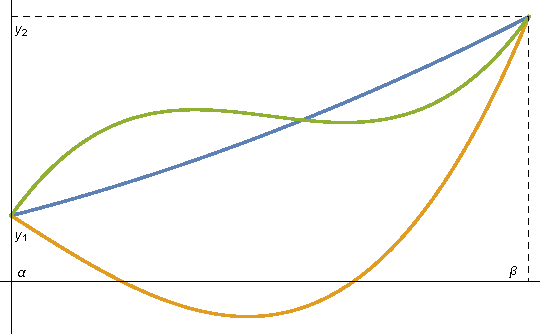
\includegraphics[width=0.5\textwidth]{Figures/fig_2_1.pdf}
    \caption{Different possible functions}
    \label{fig_2_1}
\end{figure}
We assume that the extremum exists, \(y = y(x)\), and consider small perturbation \(y \to y + \epsilon \eta(x)\) with \(\eta\) satisfying \(\eta(\alpha) = \eta(\beta) = 0\). We want to compute \(F[y + \epsilon \eta]\).

\begin{lemma}{Fundemental Lemma of Calculus of Variations}{}
    If \(g: [\alpha, \beta] \to \mathbb{R}\) is continuous on \([\alpha, \beta]\) and \(\int_\alpha^\beta g(x) \cdot \eta(x) \dif x = 0\) for all \(\eta\) continuous on \([\alpha, \beta]\) with \(\eta(\alpha) = \eta(\beta) = 0\), then \(g = 0\) on \([\alpha, \beta]\).
\end{lemma}
\begin{proof}
    Assume otherwise, \(\exists \overline{x} \in (\alpha, \beta)\) such that \(g(\overline{x}) \neq 0\). Without loss of generality, \(g(\overline{x}) > 0\), then there exists interval \([x_1, x_2] \subseteq (\alpha, \beta)\) such that \(f(x) > c > 0\) for \(x \in [x_1, x_2]\) and some \(c\). Take
    \begin{equation}
        \eta(x) = \begin{dcases}
            (x-x_1)(x_2 - x), &\text{ if } x \in [x_1, x_2]\\
            0, &\text{ otherwise} \\
        \end{dcases}.
    \end{equation}
    So
    \[
        \int^\beta_\alpha g(x) \eta(x) \dif x > c \int^{x_2}_{x_1} (x - x_1)(x_2 - x) \dif x > 0.
    \]
\end{proof}
\begin{remark}
    The function \(\eta\) is an example of a bump function. There are \(C^k\) bump functions
    \[
        \eta(x) = \begin{dcases}
            ((x-x_1)(x_2 - x))^{k + 1}, &\text{ if } x \in [x_1, x_2]\\
            0, &\text{ otherwise} \\
        \end{dcases}.
    \]
\end{remark}
Now we go back to \cref{eleq}.
\begin{align*}
    F[y + \epsilon \eta] &= \int_\alpha^\beta f(x, y + \epsilon \eta, y' + \epsilon \eta') \dif x\\
    &= F[y] + \epsilon \int_\alpha^\beta \pd{f}{y} \eta + \pd{f}{y'} \eta' \dif x + \mathcal{O}(\epsilon^2)\\
    &= F[y] + \epsilon\paren{\int_\alpha^\beta \pd{f}{y} \eta - \od{}{x}\paren{\pd{f}{y'}}\eta \dif x + \eval{\pd{f}{y'}\eta}_\beta^\alpha}
\end{align*}
At the extremum, we have \(F[y + \epsilon \eta] = F[y] + \mathcal{O}(\epsilon^2)\); that is, when \(\eval{\pd{F}{\epsilon}}_{\epsilon = 0} = 0\). So
\[
    \int_\alpha^\beta \paren{\pd{f}{y} - \od{}{x}\paren{\pd{f}{y'}}} \eta \dif x.
\]
By Lemma, we know
\begin{equation}
    \od{}{x}\paren{\pd{f}{y'}} - \pd{f}{y} = 0.
    \label{eulerlag}
\end{equation}
This is the Euler-Lagrange equation, and it is a necessary condition for an extremum.

\begin{remark}
    \begin{enumerate}
        \item \Cref{eulerlag} is a second order ODE for \(y(x)\) with boundary conditions \(y(\alpha) = y_1\) and \(y(\beta) = y_2\).
        \item The left-hand side of \cref{eulerlag} is denoted \(\frac{\delta F}{\delta y(x)}\), and called \textit{functional derivative}. Some books use \(\delta y = \epsilon \eta(x)\) as small variation.
        \item There are other boundary conditions possible. For example, \(\eval{\pd{f}{y'}}_{\alpha, \beta} = 0\).
        \item One needs to be careful with derivatives. \(\pd{f}{y} = \paren{\pd{f}{y}}_{x, y'}\) treating \(x, y, y'\) as independent, and the \textit{total derivative} is
        \begin{align*}
            \od{h}{x} &= \pd{h}{x} + \pd{h}{y}y' + \pd{h}{y'}y''\\
            \od{}{x} &= \pd{}{x} + y'\pd{}{y} + y'' \pd{}{y'}.
        \end{align*}
    \end{enumerate}
\end{remark}
\begin{example}
    If \(f = x\cdot ((y')^2 - y^2)\), then
    \[
        \partial_x f = (y')^2 - y^2,\quad \partial_y f = - 2xy, \quad \partial_{y'} f =2xy'.
    \]
    So \(\od{f}{x} = (y')^2 - y^2 - 2xyy' + 2xy'y''\).
\end{example}
\subsection{First Integrals of the Euler-Lagrange Equations}
In some cases \cref{eulerlag} (second order ODE) can be integrated once to a first order ODE called the \textit{first integral}.

If \(f\) does not explicitly depend on \(y\), that is, \(\pd{f}{y} = 0\). Then \cref{eulerlag} gives \(\od{}{x}\paren{\pd{f}{y'}} = 0\), and
\begin{equation}
    \pd{f}{y'} = \text{const}.
    \label{constb}
\end{equation}
\begin{example}
    Geodesics on \(\mathbb{R}^2\) have the functional
    \[
        F[y] = \int^\beta_\alpha \sqrt{\dif x^2 + \dif y^2} = \int_\alpha^\beta \sqrt{1 + (y')^2} \dif x.
    \]
    By \cref{constb}, we must have \(\pd{f}{y'} = \frac{y'}{\sqrt{1 + (y')^2}} = \text{const}\). So \(y'\) is constant, calling it \(m\). We have \(y = mx + c\), a straight line.
\end{example}